\documentclass[11pt,]{article}
\usepackage{lmodern}
\usepackage{amssymb,amsmath}
\usepackage{ifxetex,ifluatex}
\usepackage{fixltx2e} % provides \textsubscript
\ifnum 0\ifxetex 1\fi\ifluatex 1\fi=0 % if pdftex
  \usepackage[T1]{fontenc}
  \usepackage[utf8]{inputenc}
\else % if luatex or xelatex
  \ifxetex
    \usepackage{mathspec}
  \else
    \usepackage{fontspec}
  \fi
  \defaultfontfeatures{Ligatures=TeX,Scale=MatchLowercase}
\fi
% use upquote if available, for straight quotes in verbatim environments
\IfFileExists{upquote.sty}{\usepackage{upquote}}{}
% use microtype if available
\IfFileExists{microtype.sty}{%
\usepackage{microtype}
\UseMicrotypeSet[protrusion]{basicmath} % disable protrusion for tt fonts
}{}
\usepackage[margin = 1.5in]{geometry}
\usepackage{hyperref}
\PassOptionsToPackage{usenames,dvipsnames}{color} % color is loaded by hyperref
\hypersetup{unicode=true,
            pdftitle={ARMA GARCH Processes},
            pdfauthor={Abhinav Anand, IIMB},
            colorlinks=true,
            linkcolor=blue,
            citecolor=magenta,
            urlcolor=red,
            breaklinks=true}
\urlstyle{same}  % don't use monospace font for urls
\usepackage{color}
\usepackage{fancyvrb}
\newcommand{\VerbBar}{|}
\newcommand{\VERB}{\Verb[commandchars=\\\{\}]}
\DefineVerbatimEnvironment{Highlighting}{Verbatim}{commandchars=\\\{\}}
% Add ',fontsize=\small' for more characters per line
\usepackage{framed}
\definecolor{shadecolor}{RGB}{248,248,248}
\newenvironment{Shaded}{\begin{snugshade}}{\end{snugshade}}
\newcommand{\KeywordTok}[1]{\textcolor[rgb]{0.13,0.29,0.53}{\textbf{#1}}}
\newcommand{\DataTypeTok}[1]{\textcolor[rgb]{0.13,0.29,0.53}{#1}}
\newcommand{\DecValTok}[1]{\textcolor[rgb]{0.00,0.00,0.81}{#1}}
\newcommand{\BaseNTok}[1]{\textcolor[rgb]{0.00,0.00,0.81}{#1}}
\newcommand{\FloatTok}[1]{\textcolor[rgb]{0.00,0.00,0.81}{#1}}
\newcommand{\ConstantTok}[1]{\textcolor[rgb]{0.00,0.00,0.00}{#1}}
\newcommand{\CharTok}[1]{\textcolor[rgb]{0.31,0.60,0.02}{#1}}
\newcommand{\SpecialCharTok}[1]{\textcolor[rgb]{0.00,0.00,0.00}{#1}}
\newcommand{\StringTok}[1]{\textcolor[rgb]{0.31,0.60,0.02}{#1}}
\newcommand{\VerbatimStringTok}[1]{\textcolor[rgb]{0.31,0.60,0.02}{#1}}
\newcommand{\SpecialStringTok}[1]{\textcolor[rgb]{0.31,0.60,0.02}{#1}}
\newcommand{\ImportTok}[1]{#1}
\newcommand{\CommentTok}[1]{\textcolor[rgb]{0.56,0.35,0.01}{\textit{#1}}}
\newcommand{\DocumentationTok}[1]{\textcolor[rgb]{0.56,0.35,0.01}{\textbf{\textit{#1}}}}
\newcommand{\AnnotationTok}[1]{\textcolor[rgb]{0.56,0.35,0.01}{\textbf{\textit{#1}}}}
\newcommand{\CommentVarTok}[1]{\textcolor[rgb]{0.56,0.35,0.01}{\textbf{\textit{#1}}}}
\newcommand{\OtherTok}[1]{\textcolor[rgb]{0.56,0.35,0.01}{#1}}
\newcommand{\FunctionTok}[1]{\textcolor[rgb]{0.00,0.00,0.00}{#1}}
\newcommand{\VariableTok}[1]{\textcolor[rgb]{0.00,0.00,0.00}{#1}}
\newcommand{\ControlFlowTok}[1]{\textcolor[rgb]{0.13,0.29,0.53}{\textbf{#1}}}
\newcommand{\OperatorTok}[1]{\textcolor[rgb]{0.81,0.36,0.00}{\textbf{#1}}}
\newcommand{\BuiltInTok}[1]{#1}
\newcommand{\ExtensionTok}[1]{#1}
\newcommand{\PreprocessorTok}[1]{\textcolor[rgb]{0.56,0.35,0.01}{\textit{#1}}}
\newcommand{\AttributeTok}[1]{\textcolor[rgb]{0.77,0.63,0.00}{#1}}
\newcommand{\RegionMarkerTok}[1]{#1}
\newcommand{\InformationTok}[1]{\textcolor[rgb]{0.56,0.35,0.01}{\textbf{\textit{#1}}}}
\newcommand{\WarningTok}[1]{\textcolor[rgb]{0.56,0.35,0.01}{\textbf{\textit{#1}}}}
\newcommand{\AlertTok}[1]{\textcolor[rgb]{0.94,0.16,0.16}{#1}}
\newcommand{\ErrorTok}[1]{\textcolor[rgb]{0.64,0.00,0.00}{\textbf{#1}}}
\newcommand{\NormalTok}[1]{#1}
\usepackage{graphicx,grffile}
\makeatletter
\def\maxwidth{\ifdim\Gin@nat@width>\linewidth\linewidth\else\Gin@nat@width\fi}
\def\maxheight{\ifdim\Gin@nat@height>\textheight\textheight\else\Gin@nat@height\fi}
\makeatother
% Scale images if necessary, so that they will not overflow the page
% margins by default, and it is still possible to overwrite the defaults
% using explicit options in \includegraphics[width, height, ...]{}
\setkeys{Gin}{width=\maxwidth,height=\maxheight,keepaspectratio}
\IfFileExists{parskip.sty}{%
\usepackage{parskip}
}{% else
\setlength{\parindent}{0pt}
\setlength{\parskip}{6pt plus 2pt minus 1pt}
}
\setlength{\emergencystretch}{3em}  % prevent overfull lines
\providecommand{\tightlist}{%
  \setlength{\itemsep}{0pt}\setlength{\parskip}{0pt}}
\setcounter{secnumdepth}{0}
% Redefines (sub)paragraphs to behave more like sections
\ifx\paragraph\undefined\else
\let\oldparagraph\paragraph
\renewcommand{\paragraph}[1]{\oldparagraph{#1}\mbox{}}
\fi
\ifx\subparagraph\undefined\else
\let\oldsubparagraph\subparagraph
\renewcommand{\subparagraph}[1]{\oldsubparagraph{#1}\mbox{}}
\fi

%%% Use protect on footnotes to avoid problems with footnotes in titles
\let\rmarkdownfootnote\footnote%
\def\footnote{\protect\rmarkdownfootnote}

%%% Change title format to be more compact
\usepackage{titling}

% Create subtitle command for use in maketitle
\newcommand{\subtitle}[1]{
  \posttitle{
    \begin{center}\large#1\end{center}
    }
}

\setlength{\droptitle}{-2em}

  \title{ARMA GARCH Processes}
    \pretitle{\vspace{\droptitle}\centering\huge}
  \posttitle{\par}
    \author{Abhinav Anand, IIMB}
    \preauthor{\centering\large\emph}
  \postauthor{\par}
      \predate{\centering\large\emph}
  \postdate{\par}
    \date{2018/07/31}

\linespread{1.25}
\usepackage{amsmath}

\begin{document}
\maketitle

\section{The Autocorrelation Function
(ACF)}\label{the-autocorrelation-function-acf}

The correlation between random variables \(X_1, X_2\) is a measure of
their linear dependence and is defined as:
\[\rho_{12}:= \frac{\text{cov}(X_1,X_2)}{\sqrt{\text{var}(X_1)\text{var}(X_2)}}=\frac{\sigma_{12}}{\sigma_1\sigma_2}\]

It lies between -1 and 1 and for normal random variables \(\rho_{12}=0\)
implies that the variables are independent.

If we have a sample \(\{x_{1,t}, x_{2,t}\}_{t=1}^T\) the correlation can
be consistently estimated by computing sample correlation:
\[\hat{\rho}_{12}=\frac{\hat{\sigma}_{12}}{\hat{\sigma}_1\hat{\sigma}_2}\]

For a time series \(r_t\) which is weakly stationary, the lag-\(l\)
autocorrelation function is the correlation between \(r_t\) and
\(r_{t-l}\):

\[\rho_l=\frac{\sigma_{t,t-l}}{\sigma_t\sigma_{t-l}}=\frac{\sigma_{t,t-l}}{\sigma_t^2}
=\frac{\gamma_l}{\gamma_0}\]

This follows from weak stationarity:
\(\sigma^2_t=\sigma^2_{t-l}=\gamma_0\) and
\(\text{cov}(r_t,r_{t-l})=\gamma_l\).

We claim that there is no autocorrelation if \(\rho_l=0\)
\(\forall l>0\).

To estimate the autocorrelation function of lag (say) 1, we use its
sample counterpart:

\[\hat{\rho}_1=\frac{\sum_{t=2}^T (r_t-\bar{r})(r_{t-1}-\bar{r})}{\sum_{t=1}^T (r_t-\bar{r})^2}\]

In general for lag \(l\) we consistently estimate it as:
\[\hat{\rho}_l=\frac{\sum_{t=l+1}^T (r_t-\bar{r})(r_{t-1}-\bar{r})}{\sum_{t=1}^T (r_t-\bar{r})^2}\]

The statistic \(\hat{\rho_1},\hat{\rho_2},\hdots\) is the \emph{sample
autocorrelation function} of \(r_t\) and is key to capturing the linear
dependence nature of the time series in question.

\section{Autoregressive (AR)
Processes}\label{autoregressive-ar-processes}

Perhaps last period's returns may have some significant impact on the
value of the returns this period. If so, its lag-1 autocorrelation may
be useful for predicting the current period's value:

\[r_t = \phi_0+\phi_1r_{t-1}+u_t\]

where \(u_t\) is weakly stationary with mean 0 and variance
\(\sigma^2_u\). This is simply equivalent to a regression where
\(r_{t-1}\) is the explanatory or independent variable.

It's straightforward to check the conditional mean and variance of such
a process:

\[\mathbb{E}(r_t|r_{t-1}) = \phi_0+\phi_1r_{t-1}\]
\[\text{var}(r_t|r_{t-1}) = \sigma_u^2\]

And more generally there could be defined autoregressive processes of
order \(p\) (\(AR(p)\)):

\[r_t=\phi_0+\phi_1r_{t-1}+\hdots+\phi_pr_{t-p} + u_t\]

\subsection{AR(1) processes}\label{ar1-processes}

Is the AR(1) process \(r_t=\phi_0+\phi_1r_{t-1}+u_t\) weakly stationary?
This will imply that its unconditional mean and variance must be fixed
in time and lag-\(l\) covariance must depend only on the lag length
\(l\).

\[\mathbb{E}(r_t) = \phi_0 + \phi_1\mathbb{E}(r_{t-1})+\mathbb{E}(u_t)\]
\[\mathbb{E}(r_t) = \phi_0 + \phi_1\mu\]
\[\mu = \frac{\phi_0}{1-\phi_1}\]

This clearly implies that for the mean of an AR(1) process to exist,
\(\phi_1\neq 1\) and \(\phi_0=\mu\cdot(1-\phi_1)=\mu-\mu\phi_1\).

Hence a weakly stationary AR(1) process is:
\[r_t=\mu-\mu\phi_1+\phi_1r_{t-1}+u_t\]
\[r_t-\mu=(r_{t-1}-\mu)\phi_1+u_t\]
\[r_t-\mu=((r_{t-2}-\mu)\phi_2+u_{t-1})\phi_1+u_t\] \[\vdots\]
\[r_t-\mu = u_t + \phi_1u_{t-1}+\phi_1^2u_{t-2}+\hdots\]
\[r_t=\mu+\sum_{i=0}^\infty\phi_1^i\cdot u_{t-i}\]

Additionally,

\[\text{var}(r_t)=\phi_1^2\text{var}(r_{t-1})+\sigma^2_u\]

Since for weakly stationary AR(1) processes
\(\text{var}(r_t)=\text{var}(r_{t-1})=\gamma_0\) we have
\[\gamma_0 = \frac{\sigma_u^2}{1-\phi_1^2}\]

Weak stationarity immediately implies that \(\phi_1\in(-1,1)\).

Hence taken together, for an AR(1) process to be weakly stationary it is
necessary and sufficient that \(\phi_1\in(-1,1)\);\footnote{For a
  general AR(\(p\)) process, the corresponding condition is:
  \(|\phi_1|+|\phi_2|+\hdots+|\phi_p|<1\).} and the canonical AR(1)
series can be written as: \[r_t=(1-\phi_1)\mu+\phi_1r_{t-1}+u_t\]

We can plot some hypothetical autoregressive processes by simulation via
the function \texttt{arima.sim()} included in the \texttt{stats} package
that loads by default.

\begin{Shaded}
\begin{Highlighting}[]
\CommentTok{# AR(0)}
\KeywordTok{plot}\NormalTok{(}\KeywordTok{rnorm}\NormalTok{(}\DecValTok{500}\NormalTok{, }\DecValTok{0}\NormalTok{, }\FloatTok{0.8}\NormalTok{), }\DataTypeTok{type =} \StringTok{"l"}\NormalTok{, }\DataTypeTok{col =} \StringTok{"blue"}\NormalTok{)}
\KeywordTok{abline}\NormalTok{(}\DataTypeTok{h =} \DecValTok{0}\NormalTok{)}
\end{Highlighting}
\end{Shaded}

\begin{center}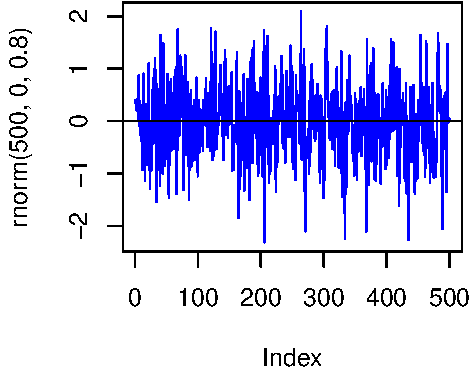
\includegraphics{FMC_T4_PhD_ARMA_GARCH_files/figure-latex/arima_sim-1} \end{center}

\begin{Shaded}
\begin{Highlighting}[]
\CommentTok{# AR(1)}
\NormalTok{ar_}\DecValTok{1}\NormalTok{ <-}\StringTok{ }\KeywordTok{arima.sim}\NormalTok{(}\DataTypeTok{n =} \DecValTok{500}\NormalTok{, }\KeywordTok{list}\NormalTok{(}\DataTypeTok{ar =} \KeywordTok{c}\NormalTok{(}\FloatTok{0.8}\NormalTok{)), }\DataTypeTok{sd =} \FloatTok{0.8}\NormalTok{)}
\KeywordTok{plot}\NormalTok{(ar_}\DecValTok{1}\NormalTok{, }\DataTypeTok{col =} \StringTok{"blue"}\NormalTok{)}
\KeywordTok{abline}\NormalTok{(}\DataTypeTok{h =} \DecValTok{0}\NormalTok{)}
\end{Highlighting}
\end{Shaded}

\begin{center}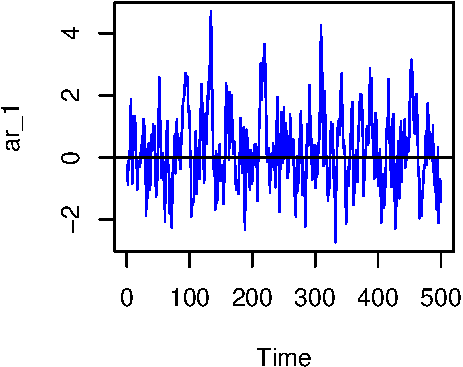
\includegraphics{FMC_T4_PhD_ARMA_GARCH_files/figure-latex/arima_sim-2} \end{center}

\begin{Shaded}
\begin{Highlighting}[]
\CommentTok{# AR(2)}
\NormalTok{ar_}\DecValTok{2}\NormalTok{ <-}\StringTok{ }\KeywordTok{arima.sim}\NormalTok{(}\DataTypeTok{n =} \DecValTok{500}\NormalTok{, }\KeywordTok{list}\NormalTok{(}\DataTypeTok{ar =} \KeywordTok{c}\NormalTok{(}\FloatTok{0.8}\NormalTok{, }\FloatTok{0.15}\NormalTok{)), }\DataTypeTok{sd =} \FloatTok{0.8}\NormalTok{)}
\KeywordTok{plot}\NormalTok{(ar_}\DecValTok{2}\NormalTok{, }\DataTypeTok{col =} \StringTok{"blue"}\NormalTok{)}
\KeywordTok{abline}\NormalTok{(}\DataTypeTok{h =} \DecValTok{0}\NormalTok{)}
\end{Highlighting}
\end{Shaded}

\begin{center}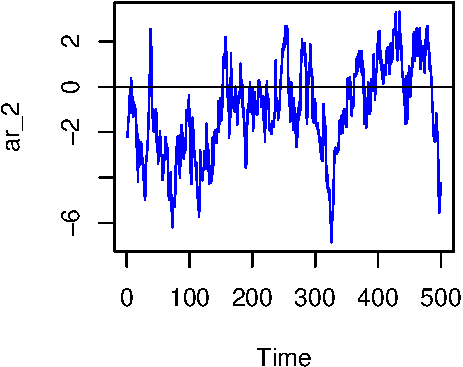
\includegraphics{FMC_T4_PhD_ARMA_GARCH_files/figure-latex/arima_sim-3} \end{center}

\begin{Shaded}
\begin{Highlighting}[]
\CommentTok{# AR(3)}
\NormalTok{ar_}\DecValTok{3}\NormalTok{ <-}\StringTok{ }\KeywordTok{arima.sim}\NormalTok{(}\DataTypeTok{n =} \DecValTok{500}\NormalTok{, }\KeywordTok{list}\NormalTok{(}\DataTypeTok{ar =} \KeywordTok{c}\NormalTok{(}\FloatTok{0.5}\NormalTok{, }\FloatTok{0.3}\NormalTok{, }\FloatTok{0.15}\NormalTok{)), }\DataTypeTok{sd =} \FloatTok{0.8}\NormalTok{)}
\KeywordTok{plot}\NormalTok{(ar_}\DecValTok{3}\NormalTok{, }\DataTypeTok{col =} \StringTok{"blue"}\NormalTok{)}
\KeywordTok{abline}\NormalTok{(}\DataTypeTok{h =} \DecValTok{0}\NormalTok{)}
\end{Highlighting}
\end{Shaded}

\begin{center}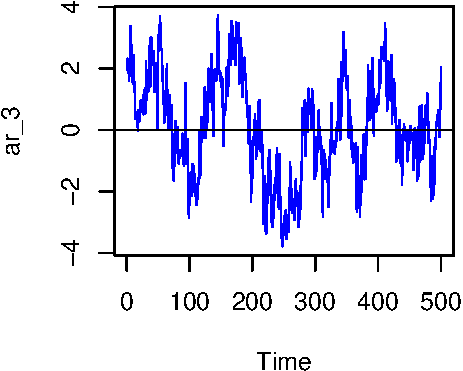
\includegraphics{FMC_T4_PhD_ARMA_GARCH_files/figure-latex/arima_sim-4} \end{center}

\subsubsection{Autocorrelation Function for AR(1)
processes}\label{autocorrelation-function-for-ar1-processes}

We can easily check that for positive lags \(l>0\), the lagged
covariance follows:

\[\gamma_l = \phi_1\gamma_{l-1}\]

Hence it follows that for the autocorrelation function
\(\rho_l = \phi_1\rho_{l-1}\); and because \(\rho_0=1\),
\(\rho_l = \phi_1^l\). This implies that the autocorrelation function of
an AR(1) series decays exponentially with rate \(\phi_1\) and starting
value 1. If \(\phi_1<0\) the series alternates between positive and
negative terms.

\textbf{Illustration}

For example let's compute the sample autocorrelation function (ACF) for
the financial market indices.

\begin{Shaded}
\begin{Highlighting}[]
\KeywordTok{acf}\NormalTok{(ret_BSE, }\DataTypeTok{na.action =}\NormalTok{ na.pass)}
\end{Highlighting}
\end{Shaded}

\begin{center}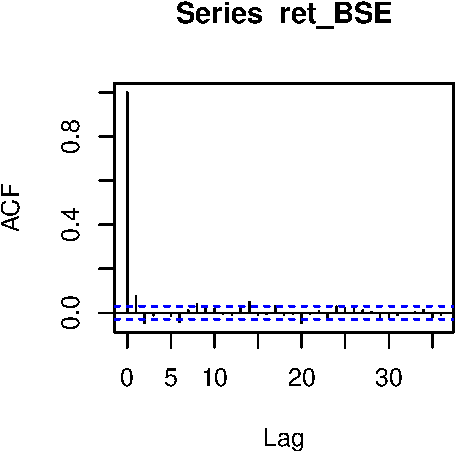
\includegraphics{FMC_T4_PhD_ARMA_GARCH_files/figure-latex/sample_ACF-1} \end{center}

\begin{Shaded}
\begin{Highlighting}[]
\KeywordTok{acf}\NormalTok{(ret_sp500, }\DataTypeTok{na.action =}\NormalTok{ na.pass)}
\end{Highlighting}
\end{Shaded}

\begin{center}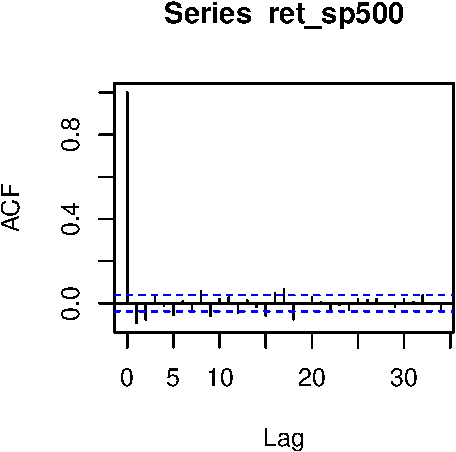
\includegraphics{FMC_T4_PhD_ARMA_GARCH_files/figure-latex/sample_ACF-2} \end{center}

\begin{Shaded}
\begin{Highlighting}[]
\KeywordTok{acf}\NormalTok{(ret_nikkei, }\DataTypeTok{na.action =}\NormalTok{ na.pass)}
\end{Highlighting}
\end{Shaded}

\begin{center}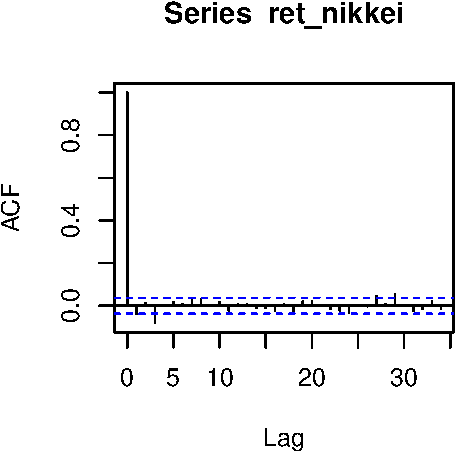
\includegraphics{FMC_T4_PhD_ARMA_GARCH_files/figure-latex/sample_ACF-3} \end{center}

What about log-returns?

\begin{Shaded}
\begin{Highlighting}[]
\NormalTok{logret_BSE <-}\StringTok{ }\KeywordTok{func_pr_to_logret}\NormalTok{(index_bse}\OperatorTok{$}\NormalTok{Close)}
\NormalTok{logret_SP <-}\StringTok{ }\KeywordTok{func_pr_to_logret}\NormalTok{(ind_sp500}\OperatorTok{$}\NormalTok{SP500)}
\NormalTok{logret_Nikkei <-}\StringTok{ }\KeywordTok{func_pr_to_logret}\NormalTok{(ind_nikkei}\OperatorTok{$}\NormalTok{NIKKEI225)}

\NormalTok{ACF_BSE <-}\StringTok{ }\KeywordTok{acf}\NormalTok{(logret_BSE, }\DataTypeTok{na.action =}\NormalTok{ na.pass)}
\end{Highlighting}
\end{Shaded}

\begin{center}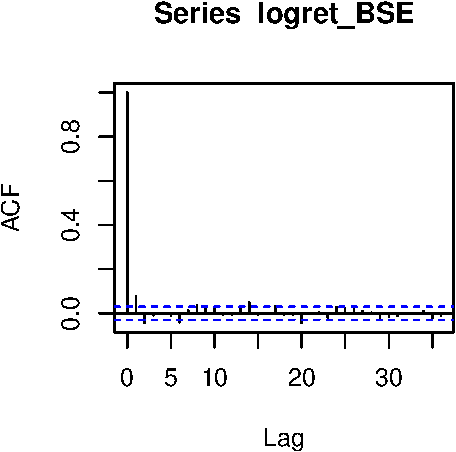
\includegraphics{FMC_T4_PhD_ARMA_GARCH_files/figure-latex/sample_ACF_logret-1} \end{center}

\begin{Shaded}
\begin{Highlighting}[]
\KeywordTok{barplot}\NormalTok{(}\KeywordTok{head}\NormalTok{(ACF_BSE}\OperatorTok{$}\NormalTok{acf))}
\end{Highlighting}
\end{Shaded}

\begin{center}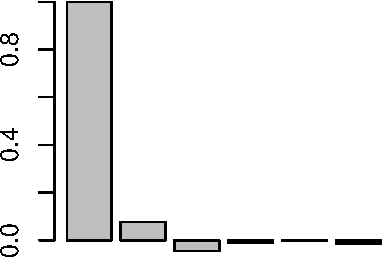
\includegraphics{FMC_T4_PhD_ARMA_GARCH_files/figure-latex/sample_ACF_logret-2} \end{center}

\begin{Shaded}
\begin{Highlighting}[]
\NormalTok{ACF_SP <-}\StringTok{ }\KeywordTok{acf}\NormalTok{(logret_SP, }\DataTypeTok{na.action =}\NormalTok{ na.pass)}
\end{Highlighting}
\end{Shaded}

\begin{center}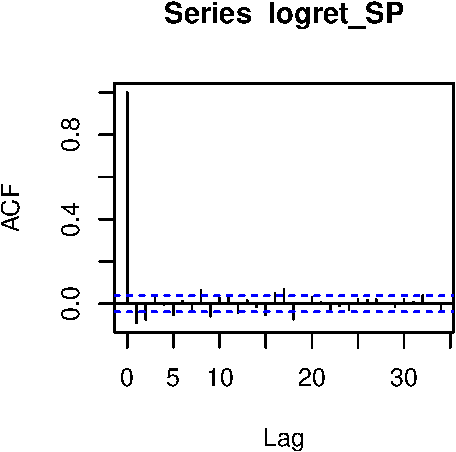
\includegraphics{FMC_T4_PhD_ARMA_GARCH_files/figure-latex/sample_ACF_logret-3} \end{center}

\begin{Shaded}
\begin{Highlighting}[]
\KeywordTok{barplot}\NormalTok{(}\KeywordTok{head}\NormalTok{(ACF_SP}\OperatorTok{$}\NormalTok{acf))}
\end{Highlighting}
\end{Shaded}

\begin{center}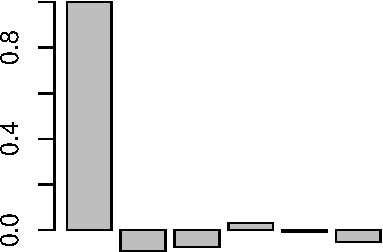
\includegraphics{FMC_T4_PhD_ARMA_GARCH_files/figure-latex/sample_ACF_logret-4} \end{center}

\begin{Shaded}
\begin{Highlighting}[]
\NormalTok{ACF_Nikkei <-}\StringTok{ }\KeywordTok{acf}\NormalTok{(logret_Nikkei, }\DataTypeTok{na.action =}\NormalTok{ na.pass)}
\end{Highlighting}
\end{Shaded}

\begin{center}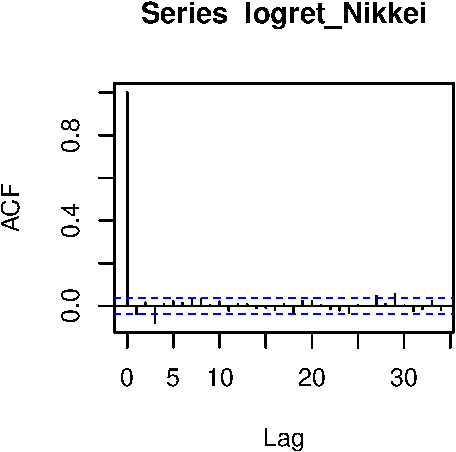
\includegraphics{FMC_T4_PhD_ARMA_GARCH_files/figure-latex/sample_ACF_logret-5} \end{center}

\begin{Shaded}
\begin{Highlighting}[]
\KeywordTok{barplot}\NormalTok{(}\KeywordTok{head}\NormalTok{(ACF_Nikkei}\OperatorTok{$}\NormalTok{acf))}
\end{Highlighting}
\end{Shaded}

\begin{center}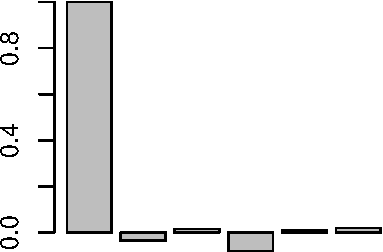
\includegraphics{FMC_T4_PhD_ARMA_GARCH_files/figure-latex/sample_ACF_logret-6} \end{center}

\subsubsection{Partial Autocorrelation Functions
(PACF)}\label{partial-autocorrelation-functions-pacf}

Is there a way to know how many lags to include for an autoregressive
return series? This issue is solved via the usage of \emph{partial
autocorrelation functions} as shown below.

Consider the following sequences of AR processes:

\[r_t=\phi_{01}+ \phi_{11}r_{t-1}+u_{1t}\]
\[r_t=\phi_{02}+ \phi_{12}r_{t-1}+\phi_{22}r_{t-2}+u_{2t}\]
\[r_t=\phi_{03}+ \phi_{13}r_{t-1}+\phi_{23}r_{t-2}+\phi_{33}r_{t-3}+u_{3t}\]
\[r_t=\phi_{04}+ \phi_{14}r_{t-1}+\phi_{24}r_{t-2}+\phi_{34}r_{t-3}+\phi_{44}r_{t-4}+u_{4t}\]
\[\vdots\]

These models are merely multiple regressions and can be estimated via
the standard least squares method.

In these models, \(\hat{\phi}_{11}\) is called the lag 1 sample PACF of
\(r_t\), \(\hat{\phi}_{22}\) of the second equation is the lag 2 sample
PACF of \(r_t\) and so on. By construction, the lag 2
\(\hat{\phi}_{22}\) is the marginal contribution of \(r_{t-2}\) in
explaining \(r_t\) over the AR(1) model and so on. Hence if the
underlying model is say AR(\(p\)) then all sample PACFs
\(\hat{\phi}_{11},\hdots, \hat{\phi}_{pp}\) must be different from 0 but
all sample PACFs from then on: \(\hat{\phi}_{p+1,p+1}, \hdots=0\). This
property can be used to find the order \(p\).

Armed with this knowledge, let's compute the PACFs for the three
financial market indices:

\begin{Shaded}
\begin{Highlighting}[]
\KeywordTok{pacf}\NormalTok{(ret_BSE, }\DataTypeTok{na.action =}\NormalTok{ na.pass)}
\end{Highlighting}
\end{Shaded}

\begin{center}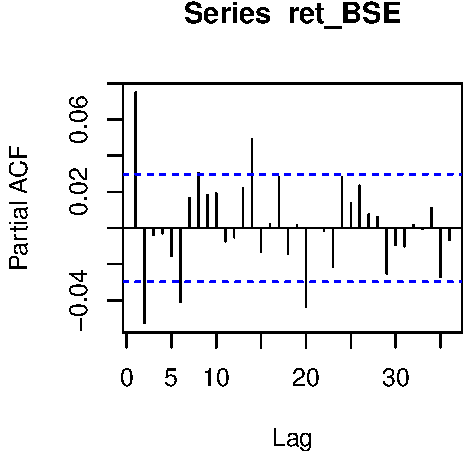
\includegraphics{FMC_T4_PhD_ARMA_GARCH_files/figure-latex/PACF-1} \end{center}

\begin{Shaded}
\begin{Highlighting}[]
\KeywordTok{pacf}\NormalTok{(ret_sp500, }\DataTypeTok{na.action =}\NormalTok{ na.pass)}
\end{Highlighting}
\end{Shaded}

\begin{center}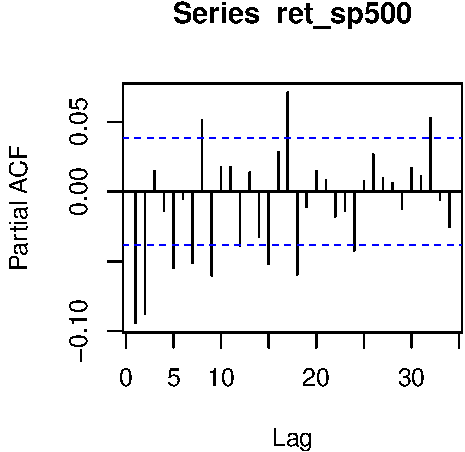
\includegraphics{FMC_T4_PhD_ARMA_GARCH_files/figure-latex/PACF-2} \end{center}

\begin{Shaded}
\begin{Highlighting}[]
\KeywordTok{pacf}\NormalTok{(ret_nikkei, }\DataTypeTok{na.action =}\NormalTok{ na.pass)}
\end{Highlighting}
\end{Shaded}

\begin{center}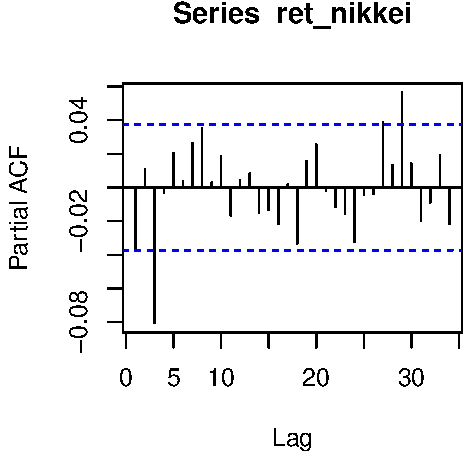
\includegraphics{FMC_T4_PhD_ARMA_GARCH_files/figure-latex/PACF-3} \end{center}

\subsubsection{Information Criteria}\label{information-criteria}

Apart from PACF, another way to find the number of lags is the use of
likelihood based information criteria. Here we look at the two most
famous ones: the Akaike Information Criterion (AIC) and the Bayesian
Information Criterion (BIC).

\[\text{AIC}(l) = -\frac{2}{T}\cdot\ln(\text{likelihood})+\frac{2}{T}\cdot(\#\text{parameters})\]

For a Gaussian AR(\(l\)),
\(AIC=\ln(\hat{\sigma}^2_{u,MLE})+2\frac{l}{T}\). The first term
measures the goodness of fit of the model while the second penalizes the
usage of parameters.

The Bayesian Information Criterion (BIC) uses a different penalty
function. For a Gaussian AR(\(l\)) is takes the following form:

\[BIC(l)=\ln(\hat{\sigma}^2_{u,MLE})+\ln(T)\cdot \frac{l}{T}\]

\section{Moving Average (MA)
Processes}\label{moving-average-ma-processes}

Consider an infinitely long autoregressive process:

\[r_t = \phi_0+\phi_1r_{t-1}+\phi_2r_{r-2}+\hdots+u_t\]

If this series is to be weakly stationary, the coefficients \(\phi_j\)
must decay sufficiently fast. One way to ensure this is to assume that
\(\phi_j=-\theta^j\) for some \(\theta\in(0,1)\).
\[r_t = \phi_0-\theta_1r_{t-1}-\theta_1^2r_{t-2}-\hdots+u_t\]
\[r_t+\sum_{j=1}^\infty \theta_1^jr_{t-j}=\phi_0+u_t\] The same form can
be written for \(r_{t-2}\):
\[r_{t-1}+\sum_{j=2}^\infty \theta_1^jr_{t-j}=\phi_0+u_{t-1}\]

Solving for the above two equations, we get:
\[r_t = \phi_0(1-\theta_1) + u_t -\theta_1u_{t-1}\]

This indicates the AR model is a weighted average of shocks
\(u_t, u_{t-1}\) and a constant. This is a \emph{moving average} form of
order 1 or MA(1). It's straightforward to check that unlike AR
processes, MA processes are \emph{always} stationary. (Can you see why?)

The general form for the MA(\(q\)) process is:
\[r_t = c_0 + u_t -\theta_1u_{t-1}-\theta_2u_{t-2}-\hdots-\theta_qu_{t-q}\]

\subsection{Autocorrelation Function}\label{autocorrelation-function}

Consider the MA(1) model with the constant term 0:

\[r_{t} = u_t -\theta_1u_{t-1}\]
\[r_{t-l}r_t = u_tr_{t-l} -\theta_1u_{t-1}r_{t-l}\]
\[\mathbb{E}(r_{t-l}r_t)=0-\theta_1\mathbb{E}(u_{t-1}r_{t-l})\] From
this we see that: \[\gamma_1=-\theta_1\sigma^2_u\] \[\gamma_{l>1}=0\]
Also, \(\text{var}(r_t) =\gamma_0= (1+\theta_1^2)\sigma_u^2\) and this
implies that for \(\rho_l = \frac{\gamma_l}{\gamma_0}\) becomes:
\[\rho_0 = 1\] \[\rho_1 = -\frac{\theta_1}{1+\theta_1^2}\]
\[\rho_{l>1} = 0\]

Hence for MA(1) processes, while the first lag autocorrelation is
nonzero, all further lags produce zero autocorrelation. This property
can be exploited to locate the order of the MA process. In general, for
an MA(\(q\)) process, the ACF cuts off at lag \(q\). Since the MA(\(q\))
process only relies on its past \(q-1\) realization, it's often called a
`finite memory' process.

To check the order of the MA series in question, we plot the ACF of the
series. If \(\rho_q\neq 0\) but \(\rho_{l>q}=0\) we may conclude that
the series is MA(\(q\)).

\subsubsection{Illustrations}\label{illustrations}

We simulate some moving average processes below:

\begin{Shaded}
\begin{Highlighting}[]
\NormalTok{n <-}\StringTok{ }\DecValTok{500}

\CommentTok{# MA(0)}
\KeywordTok{plot}\NormalTok{(}\KeywordTok{rnorm}\NormalTok{(n), }\DataTypeTok{type =} \StringTok{"l"}\NormalTok{, }\DataTypeTok{col =} \StringTok{"blue"}\NormalTok{)}
\KeywordTok{abline}\NormalTok{(}\DataTypeTok{h =} \DecValTok{0}\NormalTok{)}
\end{Highlighting}
\end{Shaded}

\begin{center}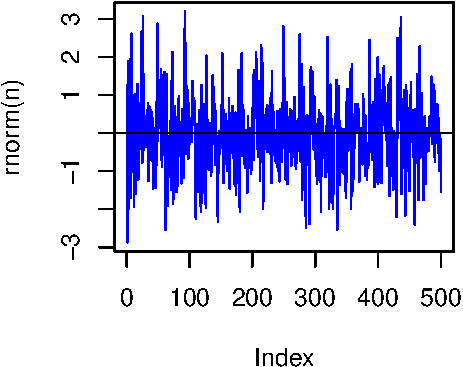
\includegraphics{FMC_T4_PhD_ARMA_GARCH_files/figure-latex/MA-1} \end{center}

\begin{Shaded}
\begin{Highlighting}[]
\CommentTok{# MA(1)}
\NormalTok{ma_}\DecValTok{1}\NormalTok{ <-}\StringTok{ }\KeywordTok{arima.sim}\NormalTok{(}\DataTypeTok{n =}\NormalTok{ n, }\KeywordTok{list}\NormalTok{(}\DataTypeTok{ma =} \KeywordTok{c}\NormalTok{(}\FloatTok{0.8}\NormalTok{)), }\DataTypeTok{innov=}\KeywordTok{rnorm}\NormalTok{(n))}
\KeywordTok{plot}\NormalTok{(ma_}\DecValTok{1}\NormalTok{, }\DataTypeTok{col =} \StringTok{"blue"}\NormalTok{)}
\KeywordTok{abline}\NormalTok{(}\DataTypeTok{h =} \DecValTok{0}\NormalTok{)}
\end{Highlighting}
\end{Shaded}

\begin{center}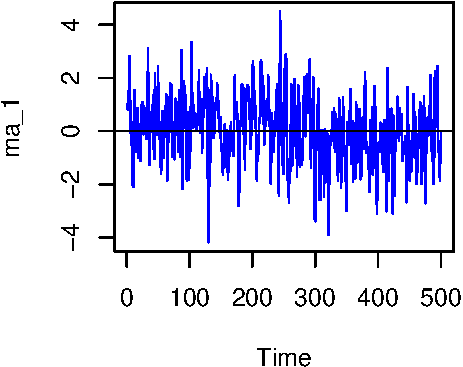
\includegraphics{FMC_T4_PhD_ARMA_GARCH_files/figure-latex/MA-2} \end{center}

\begin{Shaded}
\begin{Highlighting}[]
\KeywordTok{acf}\NormalTok{(ma_}\DecValTok{1}\NormalTok{)}
\end{Highlighting}
\end{Shaded}

\begin{center}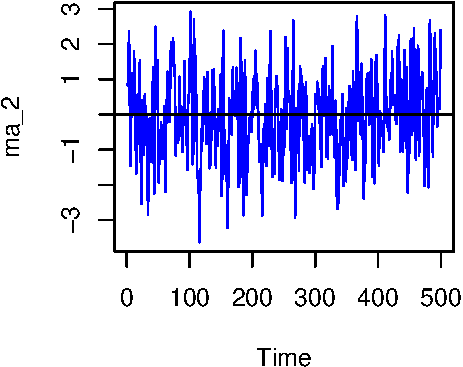
\includegraphics{FMC_T4_PhD_ARMA_GARCH_files/figure-latex/MA-3} \end{center}

\begin{Shaded}
\begin{Highlighting}[]
\CommentTok{# MA(2)}
\NormalTok{ma_}\DecValTok{2}\NormalTok{ <-}\StringTok{ }\KeywordTok{arima.sim}\NormalTok{(}\DataTypeTok{n =}\NormalTok{ n, }\KeywordTok{list}\NormalTok{(}\DataTypeTok{ma =} \KeywordTok{c}\NormalTok{(}\FloatTok{0.8}\NormalTok{, }\FloatTok{0.15}\NormalTok{)), }\DataTypeTok{innov=}\KeywordTok{rnorm}\NormalTok{(n))}
\KeywordTok{plot}\NormalTok{(ma_}\DecValTok{2}\NormalTok{, }\DataTypeTok{col =} \StringTok{"blue"}\NormalTok{)}
\KeywordTok{abline}\NormalTok{(}\DataTypeTok{h =} \DecValTok{0}\NormalTok{)}
\end{Highlighting}
\end{Shaded}

\begin{center}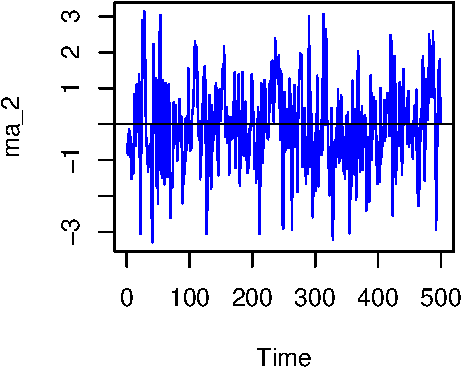
\includegraphics{FMC_T4_PhD_ARMA_GARCH_files/figure-latex/MA-4} \end{center}

\begin{Shaded}
\begin{Highlighting}[]
\KeywordTok{acf}\NormalTok{(ma_}\DecValTok{2}\NormalTok{)}
\end{Highlighting}
\end{Shaded}

\begin{center}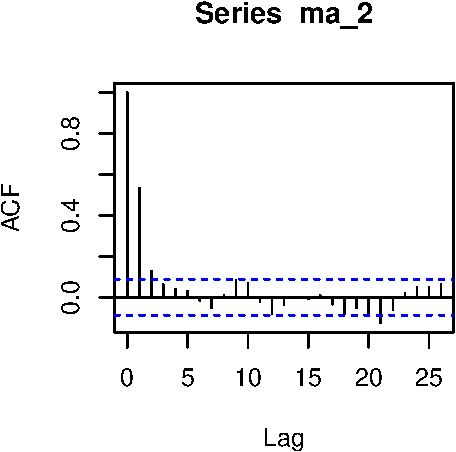
\includegraphics{FMC_T4_PhD_ARMA_GARCH_files/figure-latex/MA-5} \end{center}

\begin{Shaded}
\begin{Highlighting}[]
\CommentTok{# MA(3)}
\NormalTok{ma_}\DecValTok{3}\NormalTok{ <-}\StringTok{ }\KeywordTok{arima.sim}\NormalTok{(}\DataTypeTok{n =}\NormalTok{ n, }\KeywordTok{list}\NormalTok{(}\DataTypeTok{ma =} \KeywordTok{c}\NormalTok{(}\FloatTok{0.5}\NormalTok{, }\FloatTok{0.3}\NormalTok{, }\FloatTok{0.15}\NormalTok{)), }\DataTypeTok{innov=}\KeywordTok{rnorm}\NormalTok{(n))}
\KeywordTok{plot}\NormalTok{(ma_}\DecValTok{3}\NormalTok{, }\DataTypeTok{col =} \StringTok{"blue"}\NormalTok{)}
\KeywordTok{abline}\NormalTok{(}\DataTypeTok{h =} \DecValTok{0}\NormalTok{)}
\end{Highlighting}
\end{Shaded}

\begin{center}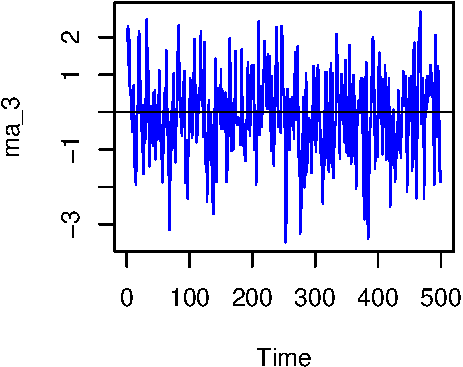
\includegraphics{FMC_T4_PhD_ARMA_GARCH_files/figure-latex/MA-6} \end{center}

\begin{Shaded}
\begin{Highlighting}[]
\KeywordTok{acf}\NormalTok{(ma_}\DecValTok{3}\NormalTok{)}
\end{Highlighting}
\end{Shaded}

\begin{center}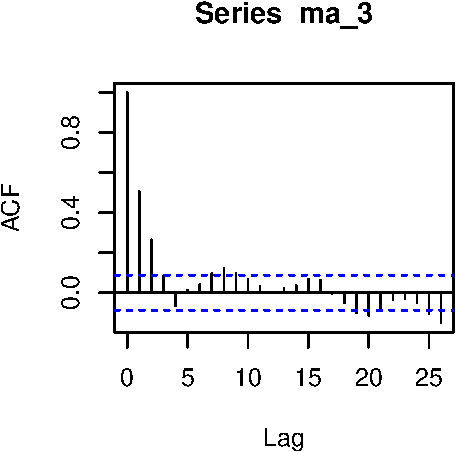
\includegraphics{FMC_T4_PhD_ARMA_GARCH_files/figure-latex/MA-7} \end{center}

\section{Autoregressive Moving Average (ARMA)
Processes}\label{autoregressive-moving-average-arma-processes}

While in principle we could fit empirical time series to AR(\(p\)) or
MA(\(q\)) models exclusively, often the concomitant order is very high.
In order to circumevent this problem, we combine AR and MA models into a
composite ARMA(\(p,q\)) model with fewer parameters to estimate.

For example the ARMA(1,1) series is as follows:
\[r_t-\phi_1r_{t-1} = \phi_0 + u_t -\theta_1u_{t-1}\]

The LHS is the AR component while the RHS is MA component.

\subsection{Properties}\label{properties}

Taking expectations we get:
\[\mathbb{E}(r_t)-\phi_1\mathbb{E}(r_{t-1}) = \phi_0 + \mathbb{E}(u_t) - \theta_1\mathbb{E}(u_{t-1})\]
\[\mathbb{E}(r_t) = \mu = \frac{\phi_0}{1-\phi_1}\]

This is the same exact mean as that of an AR(1) process. Solving for the
stationarity of the variance we get the same condition for the parameter
\(\phi_1\in (0,1)\) as that of the AR(1) model. It is not hard to derive
the autocorrelation function of the ARMA(1,1) process which behaves the
same way as that of an AR(1) process.

In general for an ARMA(\(p, q\)) process we have the following
definition:

\[r_t = \phi_0 + \sum_{i=1}^p \phi_ir_{t-i}+u_t-\sum_{j=1}^q \theta_ju_{t-j}\]

\section{Conditional Heteroskedasticity
Models}\label{conditional-heteroskedasticity-models}

In empirical time series, we do not observe volatility directly but only
estimate it with the help of some other directly observed
characteristics. However as discussed in Cont (2001) volatility displays
some striking regularities such as volatility clustering and
differential reaction to price changes.

To investigate the volatility of empirical time series, we plot the
daily returns and ACF of the Bombay stock exchange sensex.

\begin{Shaded}
\begin{Highlighting}[]
\KeywordTok{plot}\NormalTok{(logret_BSE, }\DataTypeTok{type =} \StringTok{"l"}\NormalTok{, }\DataTypeTok{col =} \StringTok{"blue"}\NormalTok{)}
\KeywordTok{abline}\NormalTok{(}\DataTypeTok{h =} \DecValTok{0}\NormalTok{)}
\end{Highlighting}
\end{Shaded}

\begin{center}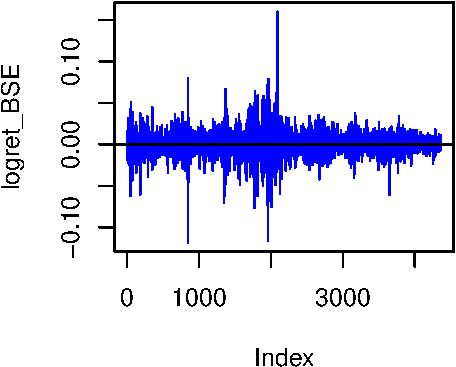
\includegraphics{FMC_T4_PhD_ARMA_GARCH_files/figure-latex/BSE_ret_ACF-1} \end{center}

\begin{Shaded}
\begin{Highlighting}[]
\KeywordTok{plot}\NormalTok{(}\KeywordTok{acf}\NormalTok{(ret_BSE, }\DataTypeTok{na.action =}\NormalTok{ na.pass))}
\end{Highlighting}
\end{Shaded}

\begin{center}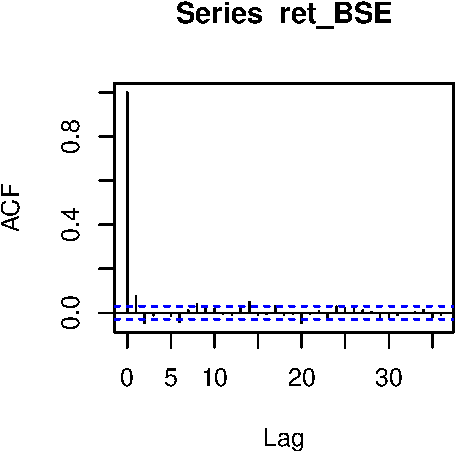
\includegraphics{FMC_T4_PhD_ARMA_GARCH_files/figure-latex/BSE_ret_ACF-2} \end{center}

While there seems to be no serial autocorrelation there is some
dependence structure embedded in the series. We can check this for
various functions of the return process such as squared returns or
absolute returns:

\begin{Shaded}
\begin{Highlighting}[]
\NormalTok{ret_BSE_sq <-}\StringTok{ }\NormalTok{ret_BSE}\OperatorTok{^}\DecValTok{2}
\KeywordTok{acf}\NormalTok{(ret_BSE_sq, }\DataTypeTok{na.action =}\NormalTok{ na.pass)}
\end{Highlighting}
\end{Shaded}

\begin{center}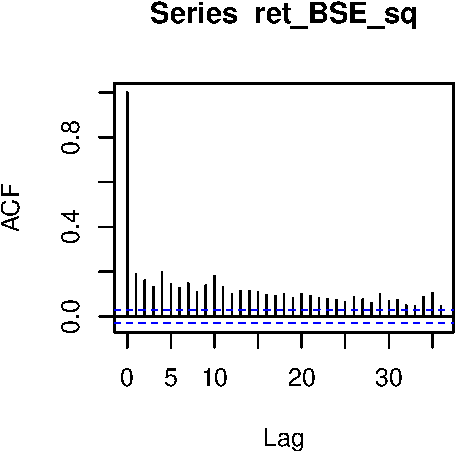
\includegraphics{FMC_T4_PhD_ARMA_GARCH_files/figure-latex/BSE_ret_ACF_sq-1} \end{center}

\begin{Shaded}
\begin{Highlighting}[]
\KeywordTok{pacf}\NormalTok{(ret_BSE_sq, }\DataTypeTok{na.action =}\NormalTok{ na.pass)}
\end{Highlighting}
\end{Shaded}

\begin{center}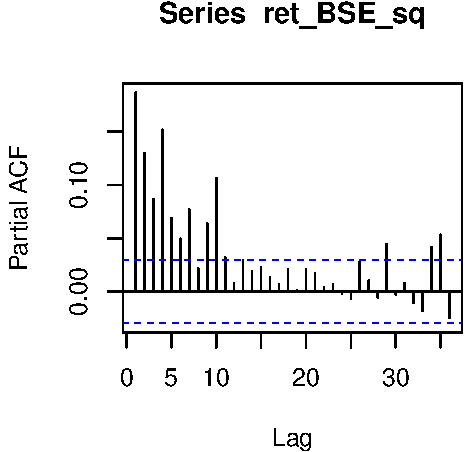
\includegraphics{FMC_T4_PhD_ARMA_GARCH_files/figure-latex/BSE_ret_ACF_sq-2} \end{center}

\begin{Shaded}
\begin{Highlighting}[]
\NormalTok{ret_BSE_abs <-}\StringTok{ }\KeywordTok{abs}\NormalTok{(ret_BSE)}
\KeywordTok{acf}\NormalTok{(ret_BSE_abs, }\DataTypeTok{na.action =}\NormalTok{ na.pass)}
\end{Highlighting}
\end{Shaded}

\begin{center}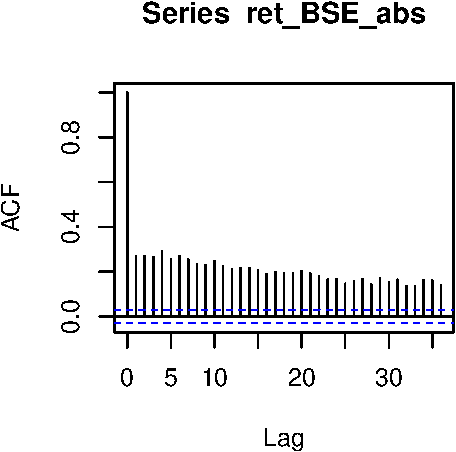
\includegraphics{FMC_T4_PhD_ARMA_GARCH_files/figure-latex/BSE_ret_ACF_sq-3} \end{center}

\begin{Shaded}
\begin{Highlighting}[]
\KeywordTok{pacf}\NormalTok{(ret_BSE_abs, }\DataTypeTok{na.action =}\NormalTok{ na.pass)}
\end{Highlighting}
\end{Shaded}

\begin{center}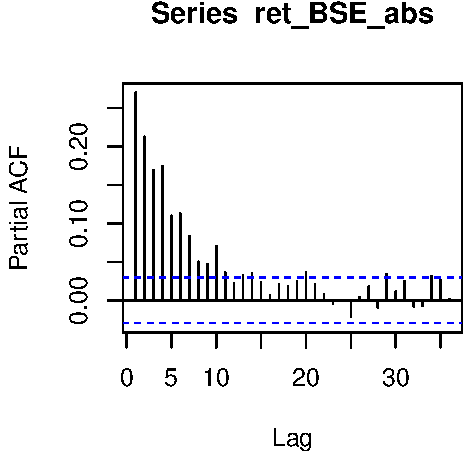
\includegraphics{FMC_T4_PhD_ARMA_GARCH_files/figure-latex/BSE_ret_ACF_sq-4} \end{center}

This behavior is also displayed by the other financial markets.

\begin{Shaded}
\begin{Highlighting}[]
\KeywordTok{acf}\NormalTok{(ret_sp500}\OperatorTok{^}\DecValTok{2}\NormalTok{, }\DataTypeTok{na.action =}\NormalTok{ na.pass)}
\end{Highlighting}
\end{Shaded}

\begin{center}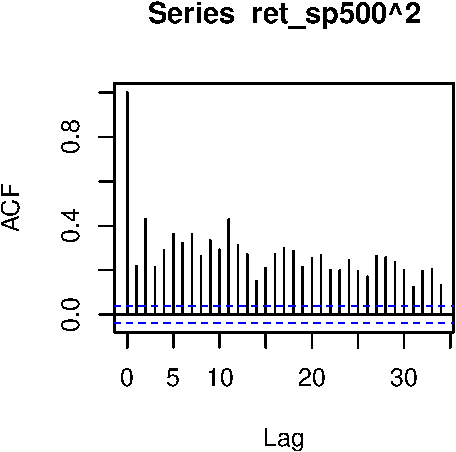
\includegraphics{FMC_T4_PhD_ARMA_GARCH_files/figure-latex/ret_ind_ACF_sq-1} \end{center}

\begin{Shaded}
\begin{Highlighting}[]
\KeywordTok{pacf}\NormalTok{(ret_sp500}\OperatorTok{^}\DecValTok{2}\NormalTok{, }\DataTypeTok{na.action =}\NormalTok{ na.pass)}
\end{Highlighting}
\end{Shaded}

\begin{center}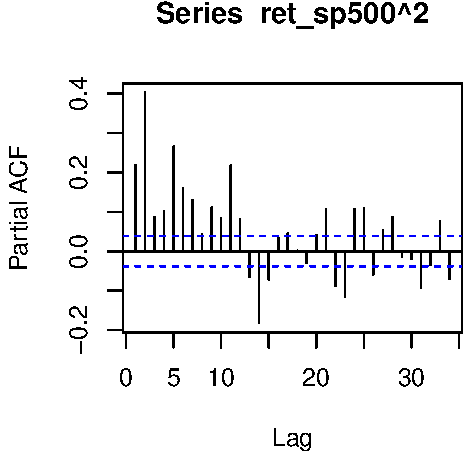
\includegraphics{FMC_T4_PhD_ARMA_GARCH_files/figure-latex/ret_ind_ACF_sq-2} \end{center}

\begin{Shaded}
\begin{Highlighting}[]
\KeywordTok{acf}\NormalTok{(ret_nikkei}\OperatorTok{^}\DecValTok{2}\NormalTok{, }\DataTypeTok{na.action =}\NormalTok{ na.pass)}
\end{Highlighting}
\end{Shaded}

\begin{center}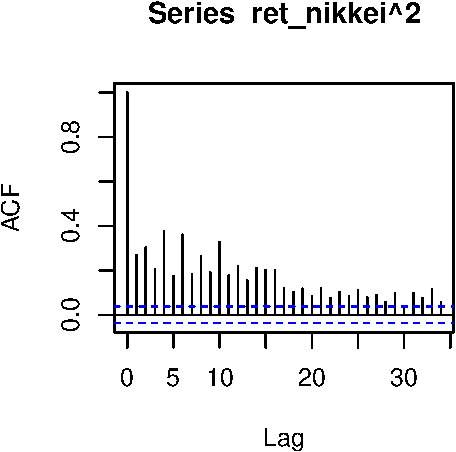
\includegraphics{FMC_T4_PhD_ARMA_GARCH_files/figure-latex/ret_ind_ACF_sq-3} \end{center}

\begin{Shaded}
\begin{Highlighting}[]
\KeywordTok{pacf}\NormalTok{(ret_nikkei}\OperatorTok{^}\DecValTok{2}\NormalTok{, }\DataTypeTok{na.action =}\NormalTok{ na.pass)}
\end{Highlighting}
\end{Shaded}

\begin{center}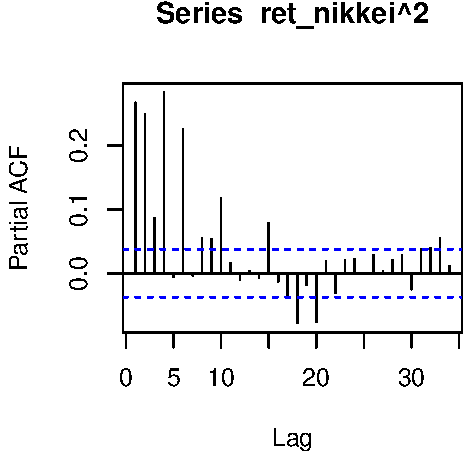
\includegraphics{FMC_T4_PhD_ARMA_GARCH_files/figure-latex/ret_ind_ACF_sq-4} \end{center}

The conditional mean volatility of the series may be written as:

\[\mu_t = \mathbb{E}(r_t|\mathbb{F}_{t-1})\]
\[\sigma_t^2 = \text{var}(r_t|\mathbb{F}_{t-1}) = \mathbb{E}((r_t-\mu_t)^2|\mathbb{F}_{t-1})
=\text{var}(u_t|\mathbb{F}_{t-1})\]

Here \(\mathbb{F}(\cdot)\) denotes the `filtration' or the information
available at the given time.

\subsection{ARCH Effect}\label{arch-effect}

Roughly speaking if the squared residuals display autocorrelation there
exist ARCH effects (autoregressive conditional heteroskedasticity
effects).

Consider \(r_t = \mu_t + u_t\). The square of the residual series
\(u_t = r_t - \mu_t\) is of interest for estimating conditional
heteroskedasticity. A popular method of testing for ARCH effects is via
the Ljung and Box statistics applied to the squared residuals series.

To test if autocorrelations of \(\{r_t\}\) are jointly 0, the
Portmanteau statistic (also called the Box-Pierce statistic) is used:
\[Q^*_m = T\cdot\sum_{l=1}^m \hat{\rho}^2_l\]

The null hypothesis is \(H_0:\rho_1=\rho_2=\hdots=\rho_m=0\) and the
alternative is that for some \(i\), \(\rho_i\neq 0\). If
\(\{r_t\}_{t=1}^T\) are iid with some moment conditions,
\(Q^*(m)\sim\chi^2(m)\).

The \emph{Ljung-Box} test statistic is based on the Portmanteau
statistic but increases its power via the following:
\[Q(m)=T(T+2)\cdot\sum_{l=1}^m \frac{\hat{\rho}_l^2}{T-l}\]

We test for ARCH effects via the function \texttt{Box.test()} including
in the \texttt{stats()} package

\begin{Shaded}
\begin{Highlighting}[]
\KeywordTok{Box.test}\NormalTok{(}\KeywordTok{rnorm}\NormalTok{(}\DecValTok{100}\NormalTok{)}\OperatorTok{^}\DecValTok{2}\NormalTok{, }\DataTypeTok{type =} \StringTok{"Ljung-Box"}\NormalTok{) }\CommentTok{#Benchmark squared normals}
\end{Highlighting}
\end{Shaded}

\begin{verbatim}
## 
##  Box-Ljung test
## 
## data:  rnorm(100)^2
## X-squared = 0.06802, df = 1, p-value = 0.7942
\end{verbatim}

\begin{Shaded}
\begin{Highlighting}[]
\KeywordTok{Box.test}\NormalTok{(ret_BSE_sq, }\DataTypeTok{type =} \StringTok{"Box-Pierce"}\NormalTok{) }\CommentTok{#Squared BSE returns}
\end{Highlighting}
\end{Shaded}

\begin{verbatim}
## 
##  Box-Pierce test
## 
## data:  ret_BSE_sq
## X-squared = 152.37, df = 1, p-value < 2.2e-16
\end{verbatim}

\begin{Shaded}
\begin{Highlighting}[]
\KeywordTok{Box.test}\NormalTok{(ret_BSE_abs, }\DataTypeTok{type =} \StringTok{"Ljung-Box"}\NormalTok{) }\CommentTok{#Absolute BSE returns}
\end{Highlighting}
\end{Shaded}

\begin{verbatim}
## 
##  Box-Ljung test
## 
## data:  ret_BSE_abs
## X-squared = 318.58, df = 1, p-value < 2.2e-16
\end{verbatim}

The same behavior is observed for the US and Japanese market indices

\begin{Shaded}
\begin{Highlighting}[]
\KeywordTok{Box.test}\NormalTok{((ret_sp500)}\OperatorTok{^}\DecValTok{2}\NormalTok{, }\DataTypeTok{type =} \StringTok{"Ljung-Box"}\NormalTok{) }
\end{Highlighting}
\end{Shaded}

\begin{verbatim}
## 
##  Box-Ljung test
## 
## data:  (ret_sp500)^2
## X-squared = 115.7, df = 1, p-value < 2.2e-16
\end{verbatim}

\begin{Shaded}
\begin{Highlighting}[]
\KeywordTok{Box.test}\NormalTok{((ret_nikkei)}\OperatorTok{^}\DecValTok{2}\NormalTok{, }\DataTypeTok{type =} \StringTok{"Ljung-Box"}\NormalTok{) }
\end{Highlighting}
\end{Shaded}

\begin{verbatim}
## 
##  Box-Ljung test
## 
## data:  (ret_nikkei)^2
## X-squared = 174.83, df = 1, p-value < 2.2e-16
\end{verbatim}

Hence we may safely conclude that the market indices in question display
ARCH effects---i.e., their squared residuals display autocorrelation.

\section{Autoregressive Conditional Heteroskedasticity
(ARCH)}\label{autoregressive-conditional-heteroskedasticity-arch}

The essential idea behind ARCH models is that while the `shock' or
`innovation' \(u_t\) is not autocorrelated, its squared lagged terms do
display autocorrelation. In other words, the ARCH(\(m\)) process
assumes:

\[u_t = \sigma_t\epsilon_t\]
\[\sigma_t^2 = \beta_0 + \beta_1u_{t-1}^2+\hdots+\beta_mu_{t-m}^2\]

Here \(\epsilon_t\) is iid with mean 0 and variance 1; and all
\(\beta_j\) are non negative, with \(\beta_0>0\). In practice it is
common to assume that the shocks \(\epsilon_t\) are from a standard
normal, standard \(T\) or some other suitable distribution. By
construction, in ARCH models, large shocks tend to be followed by other
large shocks.

\subsection{Properties of ARCH(1)
Processes}\label{properties-of-arch1-processes}

Consider the ARCH(1) model: \[u_t = \sigma_t\epsilon_t\]
\[\sigma^2_t = \beta_0 + \beta_1u_{t-1}^2\]

Clearly the unconditional mean is
\(\mathbb{E}(\mathbb{E}(u_t|\mathbb{F}_{t-1})) = 0\) and the variance is
\(\text{var}(u_t)=\mathbb{E}(\mathbb{E}(u^2_t|\mathbb{F}_{t-1})) = \beta_0+\beta_1\mathbb{E}(u_{t-1}^2)\)
and hence \[\text{var}(u_t) = \frac{\beta_0}{1-\beta_1}\]

In the same way if we compute higher moments and more specifically, the
kurtosis we find that the excess kurtosis of \(u_t\) is positive or in
other words, for an ARCH(1) process the shocks are more
fat-tailed---more likely to produce extreme values. This is consistent
with empirical observations.

\subsection{\texorpdfstring{Order Determination of ARCH(\(m\))
Processes}{Order Determination of ARCH(m) Processes}}\label{order-determination-of-archm-processes}

The ARCH(\(m\)) process is:
\[\sigma_t^2 = \beta_0+\beta_1u_{t-1}^2+\hdots+\beta_mu_{t-m}^2\]

Since \(u_t^2\) is an unbiased estimator of \(\sigma_t^2\) we can
interpret the ARCH(\(m\)) process as a special form of an AR(\(m\))
process for square errors.

If ARCH effects are deemed significant, we can employ the PACFs of
squared residuals to find the order of the ARCH series just as we did
for AR processes.

Hence we apply this idea to the market indices below.

\begin{Shaded}
\begin{Highlighting}[]
\KeywordTok{pacf}\NormalTok{(ret_BSE_sq, }\DataTypeTok{na.action =}\NormalTok{ na.pass)}
\end{Highlighting}
\end{Shaded}

\begin{center}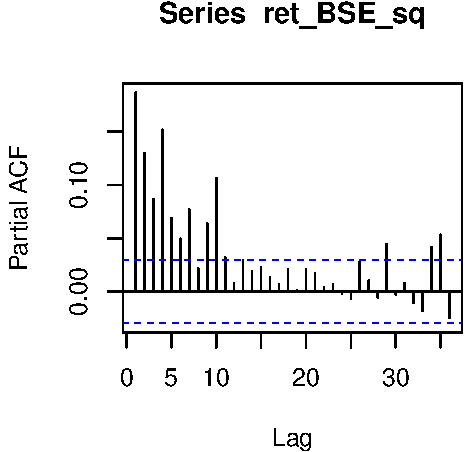
\includegraphics{FMC_T4_PhD_ARMA_GARCH_files/figure-latex/ARCH_order-1} \end{center}

\begin{Shaded}
\begin{Highlighting}[]
\KeywordTok{pacf}\NormalTok{((ret_sp500)}\OperatorTok{^}\DecValTok{2}\NormalTok{, }\DataTypeTok{na.action =}\NormalTok{ na.pass)}
\end{Highlighting}
\end{Shaded}

\begin{center}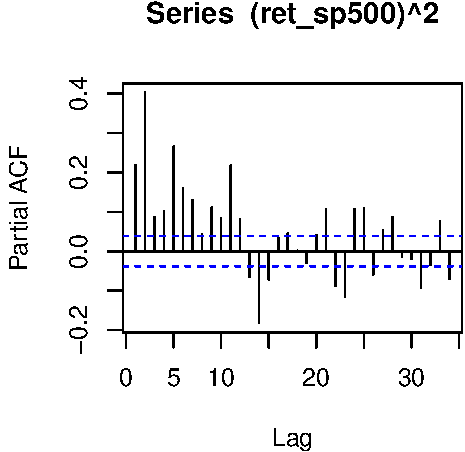
\includegraphics{FMC_T4_PhD_ARMA_GARCH_files/figure-latex/ARCH_order-2} \end{center}

\begin{Shaded}
\begin{Highlighting}[]
\KeywordTok{pacf}\NormalTok{((ret_nikkei)}\OperatorTok{^}\DecValTok{2}\NormalTok{, }\DataTypeTok{na.action =}\NormalTok{ na.pass)}
\end{Highlighting}
\end{Shaded}

\begin{center}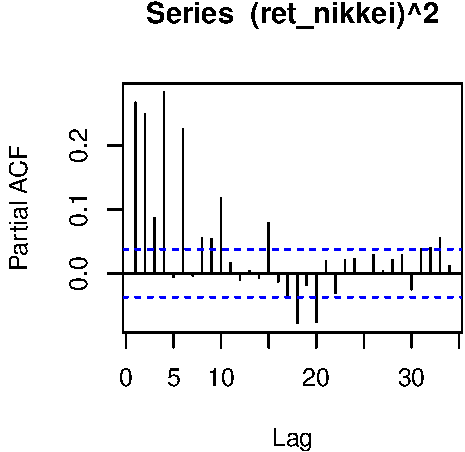
\includegraphics{FMC_T4_PhD_ARMA_GARCH_files/figure-latex/ARCH_order-3} \end{center}

Depending on the distributional assumptions for \(\epsilon_t\) we use
different forms of the maximum likelihood estimation for estimating ARCH
processes. Additionally to check if the ARCH model is well specified, we
notice that \(\tilde{u}_t = \frac{u_t}{\sigma_t}\) is an iid sequence.

\section{Generalized ARCH (GARCH)
Processes}\label{generalized-arch-garch-processes}

Usage of GARCH models can shorten the order of the corresponding ARCH
models. A GARCH(\(m,n\)) process is: \[u_t = \sigma_t \epsilon_t\]
\[\sigma_t^2 = \alpha_0 + \sum_{i=1}^m \alpha_iu_{t-i}^2 + \sum_{j=1}^n \beta_j\sigma_{t-j}^2\]

GARCH series can be thought to be ARMA series for the squared error
\(u_t^2\). GARCH models are consistent with the phenomenon of volatility
clustering and thei tail distribution is fatter than that of normals.

\section{Application: Fitting ARMA GARCH
Models}\label{application-fitting-arma-garch-models}

We check if the three financial market indices can be fitted
satisfactorily to ARMA GARCH processes.

\subsection{The Bombay Stock Exchange}\label{the-bombay-stock-exchange}

\begin{Shaded}
\begin{Highlighting}[]
\CommentTok{# For lag order indication of MA and AR resp}
\KeywordTok{acf}\NormalTok{(ret_BSE, }\DataTypeTok{na.action =}\NormalTok{ na.pass)}
\end{Highlighting}
\end{Shaded}

\begin{center}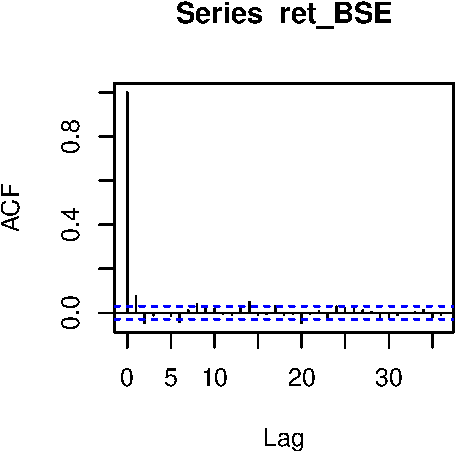
\includegraphics{FMC_T4_PhD_ARMA_GARCH_files/figure-latex/BSE_fit_ARMA_GARCH_ACF-1} \end{center}

\begin{Shaded}
\begin{Highlighting}[]
\KeywordTok{pacf}\NormalTok{(ret_BSE, }\DataTypeTok{na.action =}\NormalTok{ na.pass)}
\end{Highlighting}
\end{Shaded}

\begin{center}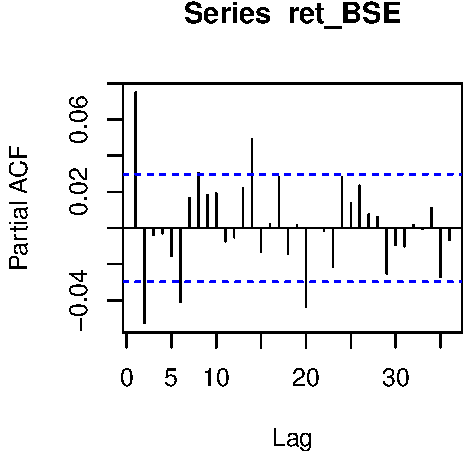
\includegraphics{FMC_T4_PhD_ARMA_GARCH_files/figure-latex/BSE_fit_ARMA_GARCH_ACF-2} \end{center}

\begin{Shaded}
\begin{Highlighting}[]
\CommentTok{# For lag order of ARCH and GARCH}
\KeywordTok{acf}\NormalTok{(ret_BSE_sq, }\DataTypeTok{na.action =}\NormalTok{ na.pass)}
\end{Highlighting}
\end{Shaded}

\begin{center}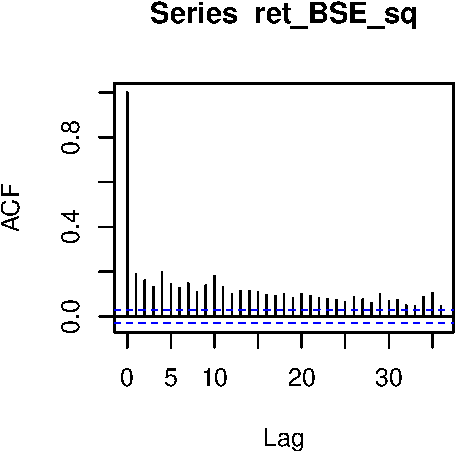
\includegraphics{FMC_T4_PhD_ARMA_GARCH_files/figure-latex/BSE_fit_ARMA_GARCH_ACF-3} \end{center}

We will use two main functions for estimating such models. One is the
function \texttt{tseries::garch()} which may be used for relatively
simple fittings and the other are sets of functions from the package
\texttt{rugarch} which offers more options including a diverse set of
distributions for the innovations.

\begin{Shaded}
\begin{Highlighting}[]
\CommentTok{# Specify an ARMA(1,1) GARCH(1,1) model}
\NormalTok{spec_garch_BSE <-}\StringTok{ }\NormalTok{rugarch}\OperatorTok{::}\KeywordTok{ugarchspec}\NormalTok{(}\DataTypeTok{variance.model=}\KeywordTok{list}\NormalTok{(}\DataTypeTok{model=}\StringTok{"sGARCH"}\NormalTok{),}
                                      \DataTypeTok{mean.model=}\KeywordTok{list}\NormalTok{(}\DataTypeTok{armaOrder=}\KeywordTok{c}\NormalTok{(}\DecValTok{1}\NormalTok{,}\DecValTok{1}\NormalTok{))}
\NormalTok{                                      )}

\CommentTok{# Estimate it}
\NormalTok{est_garch_BSE <-}\StringTok{ }\NormalTok{rugarch}\OperatorTok{::}\KeywordTok{ugarchfit}\NormalTok{(}\DataTypeTok{data =} \OperatorTok{!}\KeywordTok{is.na}\NormalTok{(ret_BSE),}
                                    \DataTypeTok{spec =}\NormalTok{ spec_garch_BSE}
\NormalTok{                                    )}

\KeywordTok{show}\NormalTok{(est_garch_BSE)}
\end{Highlighting}
\end{Shaded}

\begin{verbatim}
## 
## *---------------------------------*
## *          GARCH Model Fit        *
## *---------------------------------*
## 
## Conditional Variance Dynamics    
## -----------------------------------
## GARCH Model  : sGARCH(1,1)
## Mean Model   : ARFIMA(1,0,1)
## Distribution : norm 
## 
## Optimal Parameters
## ------------------------------------
##         Estimate  Std. Error    t value Pr(>|t|)
## mu       1.00000    0.000069 14469.4572 0.000000
## ar1      0.00000    0.149954     0.0000 1.000000
## ma1      0.24835    0.169734     1.4632 0.143417
## omega    0.00000    0.000000     4.8712 0.000001
## alpha1   0.05000    0.009027     5.5390 0.000000
## beta1    0.90000    0.001927   467.0365 0.000000
## 
## Robust Standard Errors:
##         Estimate  Std. Error    t value Pr(>|t|)
## mu       1.00000    0.000088 11357.7486  0.00000
## ar1      0.00000    0.382008     0.0000  1.00000
## ma1      0.24835    0.231867     1.0711  0.28412
## omega    0.00000    0.000000     1.4461  0.14814
## alpha1   0.05000    0.006664     7.5035  0.00000
## beta1    0.90000    0.003512   256.2781  0.00000
## 
## LogLikelihood : 24036.85 
## 
## Information Criteria
## ------------------------------------
##                     
## Akaike       -11.006
## Bayes        -10.997
## Shibata      -11.006
## Hannan-Quinn -11.003
## 
## Weighted Ljung-Box Test on Standardized Residuals
## ------------------------------------
##                         statistic p-value
## Lag[1]                      1.321  0.2504
## Lag[2*(p+q)+(p+q)-1][5]     1.392  0.9992
## Lag[4*(p+q)+(p+q)-1][9]     1.401  0.9981
## d.o.f=2
## H0 : No serial correlation
## 
## Weighted Ljung-Box Test on Standardized Squared Residuals
## ------------------------------------
##                         statistic p-value
## Lag[1]                  0.0003925  0.9842
## Lag[2*(p+q)+(p+q)-1][5] 0.0003937  1.0000
## Lag[4*(p+q)+(p+q)-1][9] 0.0003939  1.0000
## d.o.f=2
## 
## Weighted ARCH LM Tests
## ------------------------------------
##             Statistic Shape Scale P-Value
## ARCH Lag[3] 5.822e-09 0.500 2.000  0.9999
## ARCH Lag[5] 6.045e-09 1.440 1.667  1.0000
## ARCH Lag[7] 6.580e-09 2.315 1.543  1.0000
## 
## Nyblom stability test
## ------------------------------------
## Joint Statistic:  -1698.966
## Individual Statistics:              
## mu      701.92
## ar1      31.71
## ma1      34.81
## omega  1367.22
## alpha1  103.40
## beta1  1151.80
## 
## Asymptotic Critical Values (10% 5% 1%)
## Joint Statistic:          1.49 1.68 2.12
## Individual Statistic:     0.35 0.47 0.75
## 
## Sign Bias Test
## ------------------------------------
##                      t-value       prob sig
## Sign Bias          3.366e+01 5.841e-221 ***
## Negative Sign Bias 1.175e+03  0.000e+00 ***
## Positive Sign Bias 8.267e+01  0.000e+00 ***
## Joint Effect       1.668e+06  0.000e+00 ***
## 
## 
## Adjusted Pearson Goodness-of-Fit Test:
## ------------------------------------
##   group statistic p-value(g-1)
## 1    20     82257            0
## 2    30    125641            0
## 3    40    169128            0
## 4    50    212660            0
## 
## 
## Elapsed time : 0.5346069
\end{verbatim}

We can also fit standard \(T\) innovations instead of normal
innovations:

\begin{Shaded}
\begin{Highlighting}[]
\CommentTok{# Specify an ARMA(1,1) GARCH model}
\NormalTok{spec_garch_BSE <-}\StringTok{ }\NormalTok{rugarch}\OperatorTok{::}\KeywordTok{ugarchspec}\NormalTok{(}\DataTypeTok{variance.model=}\KeywordTok{list}\NormalTok{(}\DataTypeTok{model=}\StringTok{"sGARCH"}\NormalTok{),}
                                      \DataTypeTok{mean.model=}\KeywordTok{list}\NormalTok{(}\DataTypeTok{armaOrder=}\KeywordTok{c}\NormalTok{(}\DecValTok{1}\NormalTok{,}\DecValTok{1}\NormalTok{)),}
                                      \DataTypeTok{distribution.model =} \StringTok{"std"}
\NormalTok{                                      )}

\CommentTok{# Estimate it}
\NormalTok{est_garch_BSE <-}\StringTok{ }\NormalTok{rugarch}\OperatorTok{::}\KeywordTok{ugarchfit}\NormalTok{(}\DataTypeTok{data =} \OperatorTok{!}\KeywordTok{is.na}\NormalTok{(ret_BSE),}
                                    \DataTypeTok{spec =}\NormalTok{ spec_garch_BSE}
\NormalTok{                                    )}

\KeywordTok{show}\NormalTok{(est_garch_BSE)}
\end{Highlighting}
\end{Shaded}

\begin{verbatim}
## 
## *---------------------------------*
## *          GARCH Model Fit        *
## *---------------------------------*
## 
## Conditional Variance Dynamics    
## -----------------------------------
## GARCH Model  : sGARCH(1,1)
## Mean Model   : ARFIMA(1,0,1)
## Distribution : std 
## 
## Optimal Parameters
## ------------------------------------
##         Estimate  Std. Error    t value Pr(>|t|)
## mu       1.00000    0.000058 1.7246e+04 0.000000
## ar1      0.00000    0.402015 0.0000e+00 1.000000
## ma1      0.24835    0.322341 7.7046e-01 0.441024
## omega    0.00000    0.000000 4.4808e+00 0.000007
## alpha1   0.05000    0.007710 6.4854e+00 0.000000
## beta1    0.90000    0.001950 4.6162e+02 0.000000
## shape    4.00000    0.051517 7.7645e+01 0.000000
## 
## Robust Standard Errors:
##         Estimate  Std. Error    t value Pr(>|t|)
## mu       1.00000    0.000130 7675.49295 0.000000
## ar1      0.00000    0.356266    0.00000 1.000000
## ma1      0.24835    0.183749    1.35159 0.176507
## omega    0.00000    0.000000    0.99992 0.317347
## alpha1   0.05000    0.023766    2.10381 0.035395
## beta1    0.90000    0.005188  173.49298 0.000000
## shape    4.00000    0.006755  592.16490 0.000000
## 
## LogLikelihood : 25313.9 
## 
## Information Criteria
## ------------------------------------
##                     
## Akaike       -11.590
## Bayes        -11.580
## Shibata      -11.590
## Hannan-Quinn -11.586
## 
## Weighted Ljung-Box Test on Standardized Residuals
## ------------------------------------
##                         statistic p-value
## Lag[1]                      1.321  0.2503
## Lag[2*(p+q)+(p+q)-1][5]     1.393  0.9992
## Lag[4*(p+q)+(p+q)-1][9]     1.402  0.9981
## d.o.f=2
## H0 : No serial correlation
## 
## Weighted Ljung-Box Test on Standardized Squared Residuals
## ------------------------------------
##                         statistic p-value
## Lag[1]                  0.0003925  0.9842
## Lag[2*(p+q)+(p+q)-1][5] 0.0003937  1.0000
## Lag[4*(p+q)+(p+q)-1][9] 0.0003939  1.0000
## d.o.f=2
## 
## Weighted ARCH LM Tests
## ------------------------------------
##             Statistic Shape Scale P-Value
## ARCH Lag[3] 5.822e-09 0.500 2.000  0.9999
## ARCH Lag[5] 6.044e-09 1.440 1.667  1.0000
## ARCH Lag[7] 6.580e-09 2.315 1.543  1.0000
## 
## Nyblom stability test
## ------------------------------------
## Joint Statistic:  -5023.538
## Individual Statistics:              
## mu       46.12
## ar1      16.64
## ma1      18.54
## omega  1353.46
## alpha1  101.01
## beta1  1151.79
## shape  1301.00
## 
## Asymptotic Critical Values (10% 5% 1%)
## Joint Statistic:          1.69 1.9 2.35
## Individual Statistic:     0.35 0.47 0.75
## 
## Sign Bias Test
## ------------------------------------
##                      t-value      prob sig
## Sign Bias          2.005e+01 1.221e-85 ***
## Negative Sign Bias 1.152e+03 0.000e+00 ***
## Positive Sign Bias 7.698e+01 0.000e+00 ***
## Joint Effect       1.446e+06 0.000e+00 ***
## 
## 
## Adjusted Pearson Goodness-of-Fit Test:
## ------------------------------------
##   group statistic p-value(g-1)
## 1    20     82196            0
## 2    30    125454            0
## 3    40    168789            0
## 4    50    212138            0
## 
## 
## Elapsed time : 1.540517
\end{verbatim}

\section*{References}\label{references}
\addcontentsline{toc}{section}{References}

\hypertarget{refs}{}
\hypertarget{ref-Cont:2001}{}
Cont, Rama. 2001. ``Empirical Properties of Asset Returns: Stylized
Facts and Statistical Issues.'' \emph{Quantitative Finance} 1 (2):
223--36.

\hypertarget{ref-Jondeau_Poon_Rockinger:2007}{}
Jondeau, Eric, Ser-Huang Poon, and Michael Rockinger. 2007.
\emph{Financial Modeling Under Non-Gaussian Distributions}. Springer
Finance.

\hypertarget{ref-Tsay:2010}{}
Tsay, Ruey S. 2010. \emph{Analysis of Financial Time Series}. Third
Edition. John Wiley; Sons.


\end{document}
